\subsection{Silent Token Refresh Mechanism}
This mechanism details the lifecycle of every authenticated network request and illustrates how the application seamlessly recovers when an access token has expired, keeping the user signed in without manual intervention.

\begin{figure}[H]
    \centering
    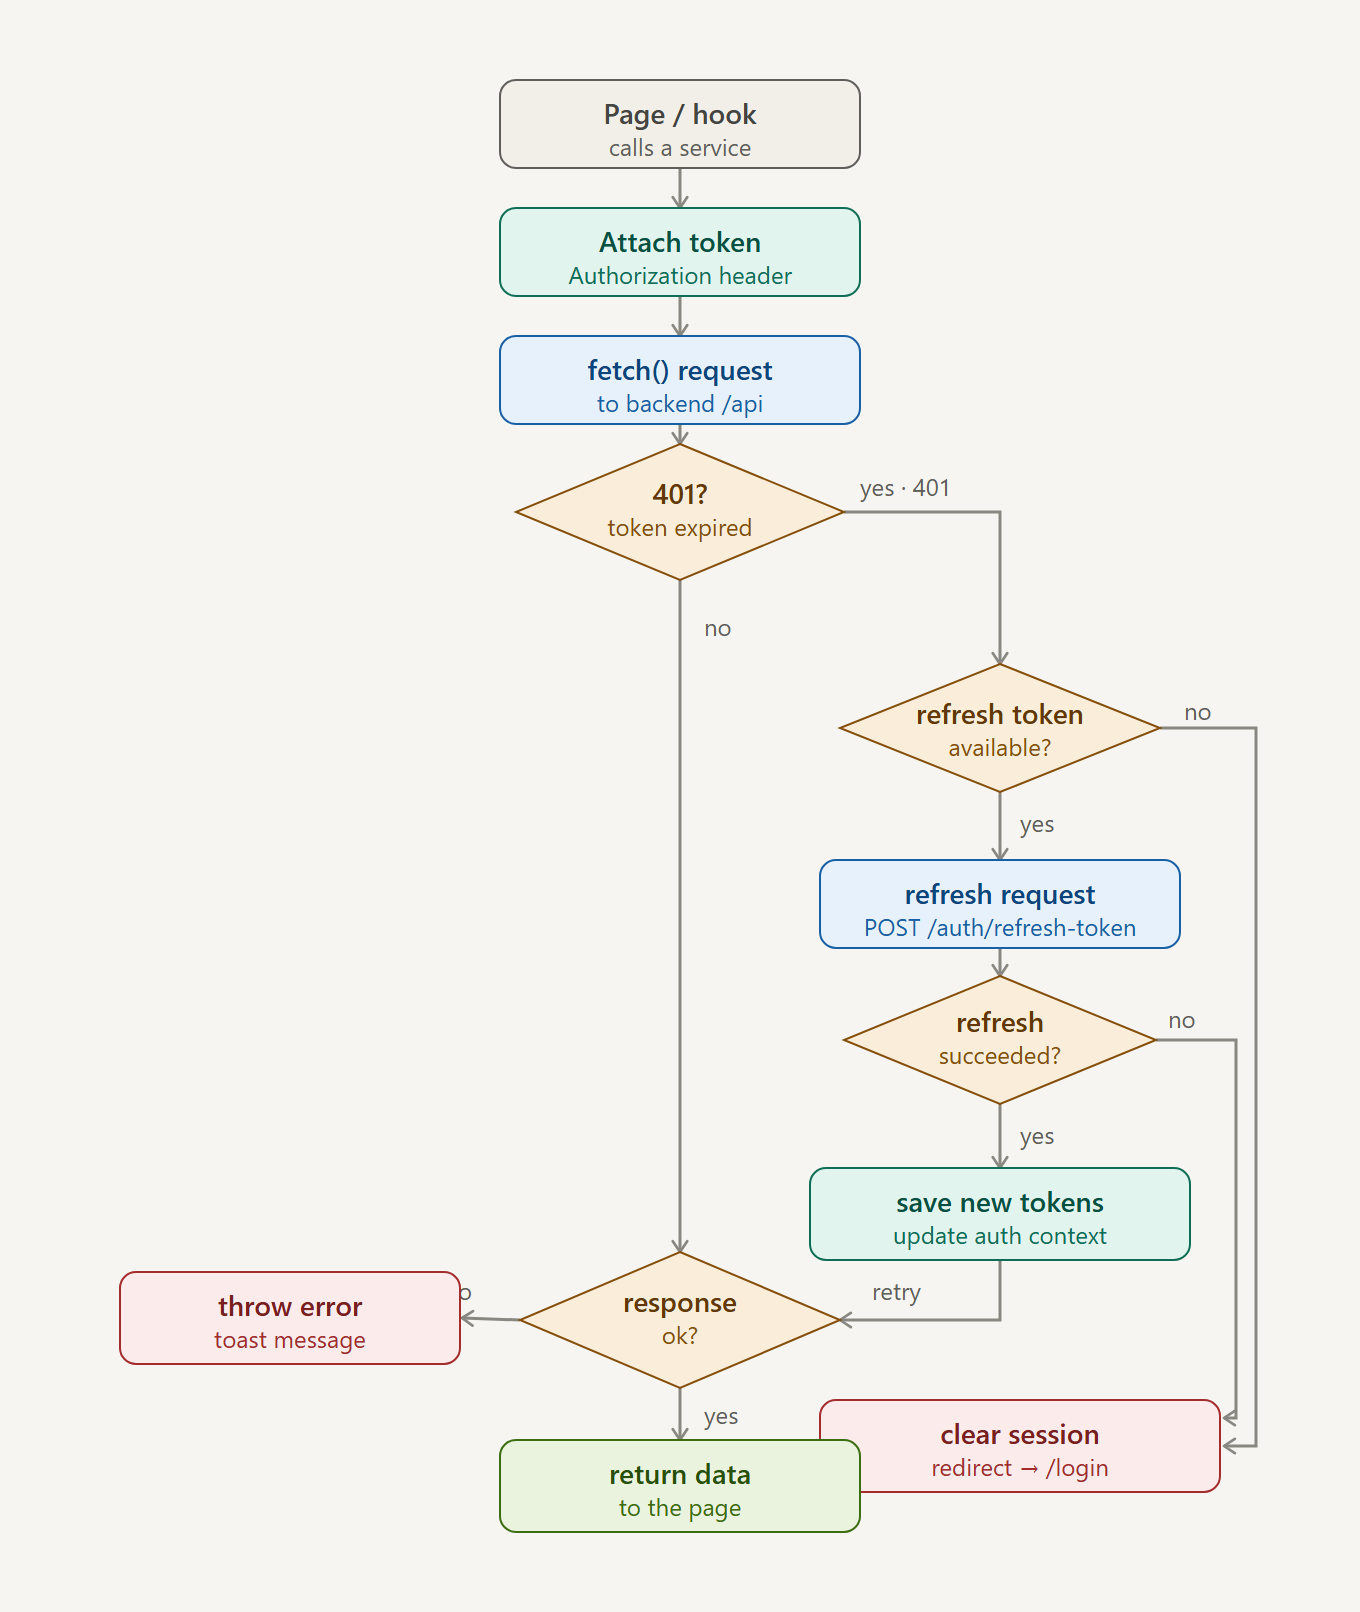
\includegraphics[width=\textwidth]{images/project-structure/project-structure3-image.png}
    \caption{Frontend Architecture and Project Structure Image}
\end{figure}

\subsubsection{Authentication Request Flow}

\textbf{Purpose:} Defines the systematic process of attaching authentication credentials to backend requests and elegantly handling \texttt{401 Unauthorized} responses via a background token refresh cycle.

\vspace{0.2cm}
\noindent\textbf{Execution Sequence:}
\begin{enumerate}
    \item \textbf{Service Invocation:} A user-facing page or custom hook triggers a network call to a designated API service.
    \item \textbf{Token Attachment:} The targeted service intercepts the outgoing request and securely attaches the current access token to the HTTP \texttt{Authorization} header.
    \item \textbf{Request Dispatch:} The service executes the \texttt{fetch()} request, routing it to the target backend \texttt{/api} endpoint.
    \item \textbf{Authorization Evaluation:} The client evaluates the backend response specifically for a \texttt{401 Unauthorized} HTTP status (indicating access token expiration):
    \begin{itemize}
        \item \textbf{If No (Success or Non-Auth Error):} The request proceeds normally. If the response is OK, the service resolves and returns the data to the page. Otherwise, it throws a standard error (typically rendered to the user as a toast notification).
        \item \textbf{If Yes (Token Expired):} The application suspends the request failure and immediately initiates the token recovery protocol.
    \end{itemize}
    \item \textbf{Refresh Token Validation:} The recovery protocol checks the client state for the presence of a refresh token:
    \begin{itemize}
        \item \textbf{If Unavailable:} The session is completely cleared, and the user is force-redirected to the \texttt{/login} route.
        \item \textbf{If Available:} The client halts the original request flow and dispatches a background refresh payload via \texttt{POST /auth/refresh-token}.
    \end{itemize}
    \item \textbf{Refresh Resolution:} The client evaluates the outcome of the refresh request:
    \begin{itemize}
        \item \textbf{If Failed:} The refresh token is also invalid or expired. The session is purged, and the user is redirected to \texttt{/login}.
        \item \textbf{If Succeeded:} The client extracts the newly generated tokens, updates the global authentication context, and seamlessly retries the original intercepted request, subsequently returning the fetched data back to the interface.
    \end{itemize}
\end{enumerate}

\vspace{0.2cm}
\noindent\textbf{Notes:}
\begin{itemize}
    \item \textbf{Invisible Recovery:} The primary benefit of this architectural design is that access token expiration is handled completely automatically and invisibly. As long as the longer-lived refresh token remains valid, the user's intended action completes successfully without them ever noticing they were momentarily signed out.
\end{itemize}